\documentclass[a4paper,12pt]{ctexart}
\usepackage{amsmath}
\usepackage{amssymb}
\usepackage{fontspec}
\usepackage{xeCJK}
\usepackage{graphicx}
\usepackage{listings}
\usepackage{xcolor} 
\usepackage{graphicx}
\usepackage{booktabs} %绘制表格
\usepackage{geometry}
\usepackage{array}
\usepackage{longtable}
\usepackage{abstract}
\usepackage{caption}
\usepackage{subcaption}
\usepackage{abstract}
\usepackage{makecell}
\usepackage{float}
%防止表格乱跑:[H]
\usepackage{listings}
%添加代码块
\usepackage{fancyhdr} 
%导入fancyhdr包
\usepackage{threeparttable}
%给代码添加注释

\lstset{
 numbers=left, %设置行号位置
 numberstyle=\tiny, %设置行号大小
 keywordstyle=\color{blue}, %设置关键字颜色
 commentstyle=\color[cmyk]{1,0,1,0}, %设置注释颜色
 escapeinside=``, %逃逸字符(1左面的键),用于显示中文
 breaklines, %自动折行
 extendedchars=false, %解决代码跨页时,章节标题,页眉等汉字不显示的问题
 xleftmargin=1em,xrightmargin=1em, aboveskip=1em, %设置边距
 tabsize=4, %设置tab空格数
 showspaces=false %不显示空格
}

\lstset{
 columns=fixed,       
 numbers=left,                            % 在左侧显示行号
 numberstyle=\tiny\color{gray},           % 设定行号格式
 frame=none,                              % 不显示背景边框
 backgroundcolor=\color[RGB]{245,245,244},% 设定背景颜色
 keywordstyle=\color[RGB]{40,40,255},     % 设定关键字颜色
 numberstyle=\footnotesize\color{darkgray},           
 commentstyle=\it\color[RGB]{0,96,96},    % 设置代码注释的格式
 stringstyle=\rmfamily\slshape\color[RGB]{128,0,0},   
            % 设置字符串格式
 showstringspaces=false,                  % 不显示字符串中的空格
 language=matlab,                         % 设置语言
}

\setlength{\parindent}{2em} %2em代表首行缩进两个字符

\CTEXsetup[format={\large\bfseries}]{section}
\CTEXsetup[format={\normalsize\bfseries}]{subsection}
\pagestyle{headings}
\pagestyle{fancy}
% 页眉设置
\fancyhead{} % 初始化页眉
\fancyhead[L]{《数值计算方法》第四次上机}
\fancyhead[R]{3200104845}
\fancyhead[C]{朱少廷}
\fancyfoot{} % 初始化页脚
\fancyfoot[L]{}
\fancyfoot[C]{\thepage}
\renewcommand{\headrulewidth}{1.5pt}%分隔线宽度4磅

\setlength{\absleftindent}{0pt}
\setlength{\absrightindent}{0pt}


\graphicspath{{pictures/}}

% Set page size and margins
\geometry{a4paper,top=3cm,bottom=2cm,left=3cm,right=3cm,marginparwidth=1.75cm}

\begin{document}
\centerline{\Large{\textbf{第四次上机作业}}}
\section{问题叙述}
在区间$[-4,4]$上给出函数$f(x)=e^{x}$的等距节点函数值表,
用分段二次插值求$e^{x}$的近似值。要求:
\begin{itemize}
    \item 等距节点函数值表的步长$h$自行选取,需满足所得到插值
          函数在$[-4,4]$上的截断误差不超过$10^{-2}$;
    \item 画出原函数$f(x)$及插值函数在$[-4,4]$上的图像。
\end{itemize}

\section{问题解答}
\subsection{节点函数值表}
\begin{lstlisting}
%% 分段节点函数表
point_num=58; % Number of sampling points
h=8/(point_num-1); % Sampling point spacing
x_value=-4:h:4;
y_value=exp(x_value);
\end{lstlisting}
\par
程序运行后,x\_value数组中存放$x_{i}$的值,y\_value数组中对应
存放$y_{i}$的值。其中point\_num为取样点个数,h为取样点间距。
表格篇幅较大,且在报告中列意义不大,可运行程序后在工作区查看对应数据。

\subsection{二次插值实现}
\begin{figure}[H]
    \centering
    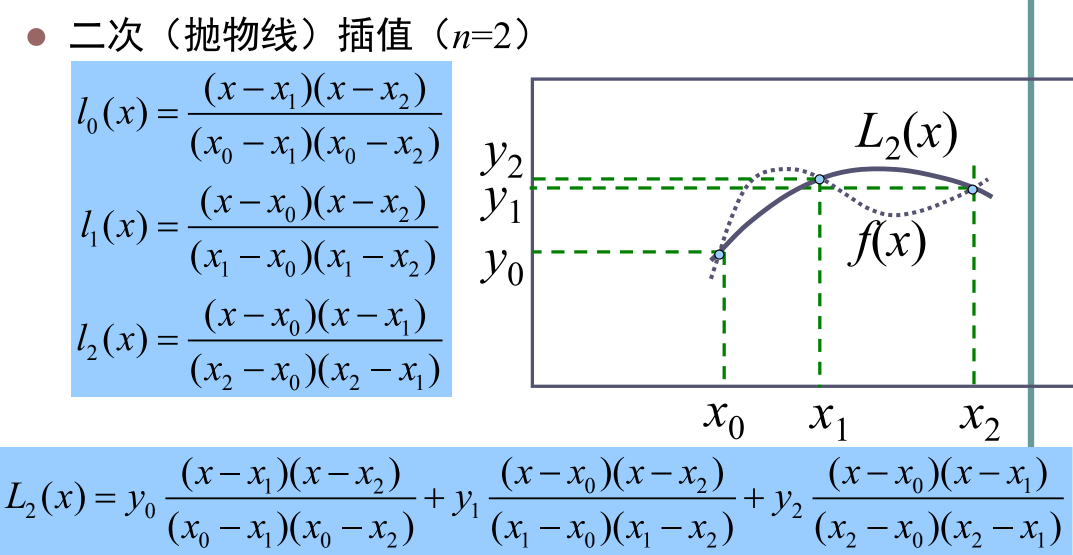
\includegraphics[width=13cm]{上机4/ercichazhi.png}
\end{figure}
\par
当求插值点$x$的插值(即求$f(x)$的近似值)时,可选取距
点$x$最近的三个插值节点$x_{i-1}$, $x_i$, $x_{i+1}$,
在小区间$[x_{i-1},x_i,x_{i+1}]$上使用二次插值公式,
称为分段抛物插值或分段二次插值。
\par
选取距$x$最近的三个差值点,即等价于寻找离x最近的$x_i$。我们之间
使用$x$坐标绝对距离来确定。即在$\frac{1}{2}(x_{i-1}+x_i)$到
$\frac{1}{2}(x_i+x_{i+1})$之间的$x$均可用$x_{i-1}$, $x_i$, $x_{i+1}$
三个节点所确定的二次函数来表示。用此方法在$[-4,4]$遍历所有x,即可
获得一条分段的二次插值函数曲线。需要注意的是,一头一尾均使用最前/最后
三个节点的二次方程来表示。
\par
实现该过程的Matlab代码如下:
\begin{lstlisting}
%% 分段二次插值
x_bond=zeros(1,length(x_value)-1); % Calculate boundary value
x_bond(1)=-4;
for i=2:length(x_value)-2
    x_bond(i)=0.5*(x_value(i)+x_value(i+1));
end
x_bond(end)=4;
count=1;
step=1e-6; % Plot sampling point spacing
x=-4:step:4;
for t=-4:step:4
    for j=1:length(x_bond)
        if t<x_bond(j)
            i=j-1;break;
        end
    end
    y0=y_value(i);y1=y_value(i+1);y2=y_value(i+2);
    x0=x_value(i);x1=x_value(i+1);x2=x_value(i+2);
    % Quadratic Lagrange interpolation
    y(count)=y0*(t-x1)*(t-x2)/(x0-x1)/(x0-x2)+y1*(t-x0)*(t-x2)/(x1-x0)/(x1-x2)+y2*(t-x0)*(t-x1)/(x2-x0)/(x2-x1);
    count=count+1;
end
\end{lstlisting}

\subsection{估算截断误差}
$R_n(x)=f(x)-P_n(x)$表示用$P_n(x)$表示$f(x)$时,在点$x$
处产生的误差。
\par
若$f(x)$在区间$[a,b]$上有直到$n+1$阶导数$f^{(n+1)}(x)$存在,
$P_n(x)$为$f(x)$在$n+1$个节点$x_i$上的$n$次插值多项式,
则$\forall x\in [a,b]$有:
\begin{figure}[H]
    \centering
    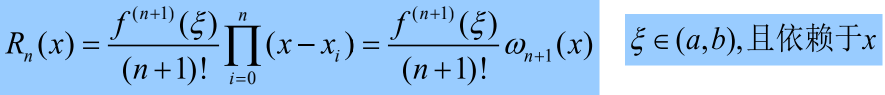
\includegraphics[width=13cm]{上机4/wucha.png}
\end{figure}
\par
设用$x_{i-1}$、$x_{i}$、$x_{i+1}$获得二次插值曲线,并设
$x=x_{i}+hs$,则
\begin{equation}
    |R_n(x)|=|\frac{e^\xi}{3!}(hs+h)(hs)(hs-h)|\leq
    |\frac{\sqrt{3}e^4h^3}{27}|\leq 0.01
\end{equation}
\par
解得:
\begin{equation}
    h\leq 0.1419
\end{equation}
\par
即:
\begin{equation}
    point\_num\geq 58
\end{equation}
使用程序验证:
\begin{lstlisting}
%% 估算截断误差
y_exp=exp(x);
Rn=abs(y-y_exp);
Rn_max=max(Rn); % Find the maximum truncation error
\end{lstlisting}
\par
可以求得当$point\_num=58$时,$R_n$的最大值为0.008598,满足小于0.01的限制。
\par
实际上,由于估算中的不等式放缩的等号并不能够取到,实际调试时发现只需要
$point\_num\geq 56$的时候就可以保证$R_n$小于0.01。

\subsection{图像绘制}
\begin{figure}[H]
    \centering
    \caption{插值后函数和原函数对比}
    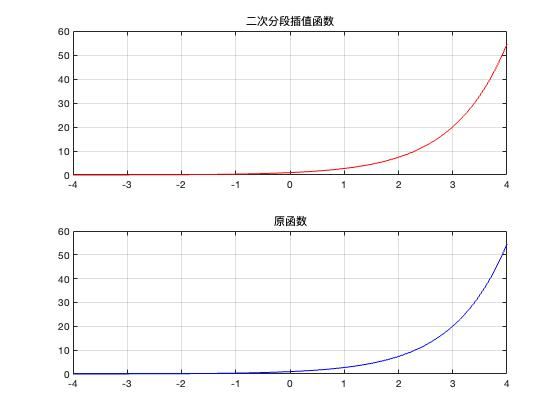
\includegraphics[width=13cm]{上机4/1.jpg}
\end{figure}
Matlab代码:
\begin{lstlisting}
%% 画图
subplot(2,1,1)
plot(x,y,'r');
grid on
syms x0;
title('二次分段插值函数')
subplot(2,1,2)
plot(x,y_exp,'b');
xlim([-4,4])
title('原函数')
grid on
\end{lstlisting}
\par
从图像中完全分辨不出原函数和插值函数的区别,说明插值后与原函数符合的
很好。

\section{小结}
\par
通过本次上机实验,我初步掌握了二次插值求函数近似值的方法。实验中
我使用理论分析与编程实践相结合的方法,用实际结果较为完美地检验了
理论结论。实验中我发现两个函数非常接近,若画在一张图上效果很不好,
因此我学习使用了subplot()函数,成功将两个函数分开画在一张图内。

\end{document}